\chapter{Background}
\label{cha:bg}

Text.


\section{Video compression concepts}
\label{sec:bg/compression}

Video is known to be one of the heaviest types of content to be stored and transmitted. Since treating uncompressed video is unfeasible, video compression or video coding formats have been developed and standardized over the years, with multiple implementations (\textit{codecs}) being released. The objective of video codecs is to limit the output data rate, measured in bits per second, while trying to maintain a perceptually good video quality.

\subsection{RGB vs Y'CbCr}
\label{sec:bg/compression/ycbcr}

The most basic form of compression can be obtained by converting individual pictures representing the video to a \textbf{color space} that better exploits human vision characteristics and then applying compression of some of the components in the new color space.

A very common color space family used in digital video and images is \textbf{Y'CbCr}, sometimes improperly called YUV (which relates to the analog domain), which exploits the fact that the human vision system is much more sensitive to light variations (brightness) than to color. The Y'CbCr color space decomposes the color information of a pixel into three components:

\begin{itemize}
    \item \textbf{Y'}: the luminance, representing the brightness of the image;
    \item \textbf{Cb}: the blue chroma component, representing a projection of the blue color;
    \item \textbf{Cr}: the red chroma component, representing a projection of the red color.
\end{itemize}

This approach is different from the common RGB (Red Green Blue) color space, where the luminance is not isolated from the color components, and allows to apply compression in a more effective way through the \textbf{chroma subsampling} technique.

Chrome subsampling refers to the practice of reducing the resolution of the chroma components while keeping the luminance at full resolution. Since our eyes are less sensitive to color than to brightness, we can reduce the color resolution by even 75\% with almost no perceptual impact on quality.

% sources from LT

The vast majority of digital video that can be found on the Internet or that is transmitted through digital television is compressed with the Y'CbCr 4:2:0 color space, the most common format for non-professional content. In Y'CbCr 4:2:0, the luminance component (Y) is encoded at full resolution, while the chroma components are stored at 1/4 of the resolution, i.e. instead of storing 8 chroma samples for every 8 pixels we only keep 2, as shown in Figure X.

% figure from LT

When compared to a typical 8-bit RGB image (equivalent to Y'CbCr 4:4:4, i.e. no subsampling), requiring 24 bits per pixel, a Y'CbCr 4:2:0 image requires only 12 bits per pixel, resulting in a 50\% saving with very similar perceived quality. When using tools like \texttt{ffmpeg}, Y'CbCr 4:2:0 is often called \texttt{yuv420p} or similar.

\subsection{Inter-frame and intra-frame compression}
\label{sec:bg/compression/intra-inter}

The major video coding standards released since the early 1990s are based on a \textbf{hybrid codec model} that exploits both temporal and spatial redundancy of videos to achieve high compression ratios.

Temporal compression, or \textbf{inter-frame compression}, relies on the fact that there is usually a high similarity between consecutive video frames. On the other hand spatial compression, or \textbf{intra-frame compression}, exploits the fact that pixels that are close to each other within a picture are usually highly correlated.

Video codecs (en\textbf{co}der/\textbf{dec}oder) are implementations of video coding standards that are able to convert the input video into a coded version in a way that is reversible, i.e. such that the decoder can reconstruct the original video with some approximation. Encoders should output a compressed representation that is as efficient as possible while trying to preserve the fidelity of the original video.

\begin{figure}[h]
	\centering
	
	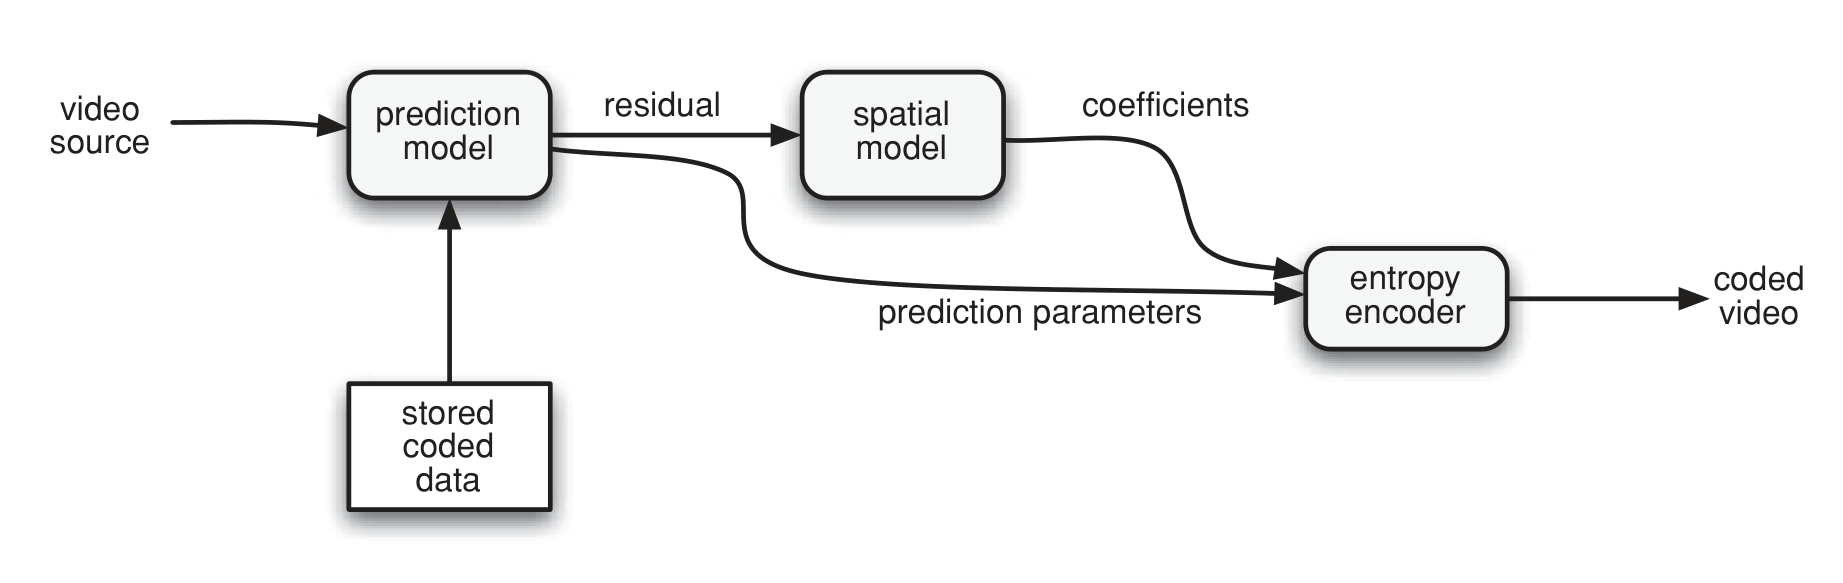
\includegraphics[width=\textwidth]{res/hybrid_codec_high_level.png}
	
	\caption{High-level hybrid codec architecture.\cite{h264}}
	\label{fig:codec_highlevel}
\end{figure}

In general, a hybrid video codec works in three phases:\cite{h264}

\begin{itemize}
    \item \textbf{Prediction model}: exploits spatial or temporal redundancy by producing a prediction of the current frame (or block of a frame) being analyzed, by looking at a previous reference frame or at other parts of the same frame. The outputs of this phase are a \textbf{residual frame}, which is the difference between the actual frame and the predicted frame, and the parameters that define how the prediction was obtained. By encoding only the residual and the parameters we can basically store only the "error" of the prediction and greatly reduce the amount of data that needs to be coded. The prediction can be obtained in two ways:
        \begin{itemize}
            \item \textbf{Temporal prediction}: in its most basic form, the prediction is the difference between the current frame and a previous (or future) reference frame. In practice, we also need to take into account the motion that occurs between frames by running a \textbf{motion estimation} algorithm that for each block\footnote{Blocks are small regions of pixels.} in the current frame finds the best matching block in the reference frame. The \textbf{motion-compensated block} becomes the prediction used to calculate the residual, which becomes the output of the prediction phase together with the \textbf{motion vectors} that explain how the prediction block was obtained (i.e. how it "moved" with respect to the reference frame).
            \item \textbf{Spatial prediction}: when encoding a block of the image, a prediction of the pixel values of the block is first calculated by looking at neighboring pixels. Statistically, pixels close to each other are expected to be similar due to spatial redundancy. Usually, this means looking at the pixels on the left and/or top edges of the block. The predicted block is then subtracted from the current block to obtain a \textbf{residual block}, which is passed onto the next phase together with the information that tells how the prediction of the block was obtained.
        \end{itemize}
        
    \item \textbf{Spatial model}: in most codecs, this phase consists in compressing the residual frame through a transform and quantization steps, followed by encoding of coefficients.
        \begin{itemize}
            \item The \textbf{transform} step often consists in applying the \textbf{Discrete Cosine Transform} (DCT) to transform the blocks in the frequency domain. The output of the DCT is a matrix of coefficients, which can be used to faithfully reconstruct the original block, although without achieving any compression.
            \item In the \textbf{quantization} step, coefficients that have insignificant impact, such as values that are close to zero, are discarded, enabling to represent the original block with some approximation by storing a smaller number of DCT coefficients (the non-discarded ones). In the decoder, the subset of coefficients can then be fed into the IDCT (the inverse of the transform), obtaining a reconstruction of the original block. The fidelity of the reconstruction depends on how strong the quantization step was, i.e. on the \textbf{quantization parameter} (QP).
            \item After quantization, the remaining coefficients are reordered through a \textbf{zigzag scan} of the matrix, making sure that the most significant coefficients are at the beginning of the sequence (a typical property of the DCT) and then encoded through \textbf{Run-Level Encoding} (RLE).
        \end{itemize}
     
    \item \textbf{Entropy coding}: in this phase all the information collected in previous phases, including quantized coefficients, quantization parameters, and motion vectors, is encoded in a bit stream. To exploit the statistical redundancy of symbols in the data, techniques like \textbf{Variable-Length Coding} (VLC), such as Huffman coding, or arithmetic coding and \textbf{Context-aware Arithmetic Encoding} (CAE) are used, achieving further compression.
\end{itemize}

\begin{figure}[hb]
	\centering
	
	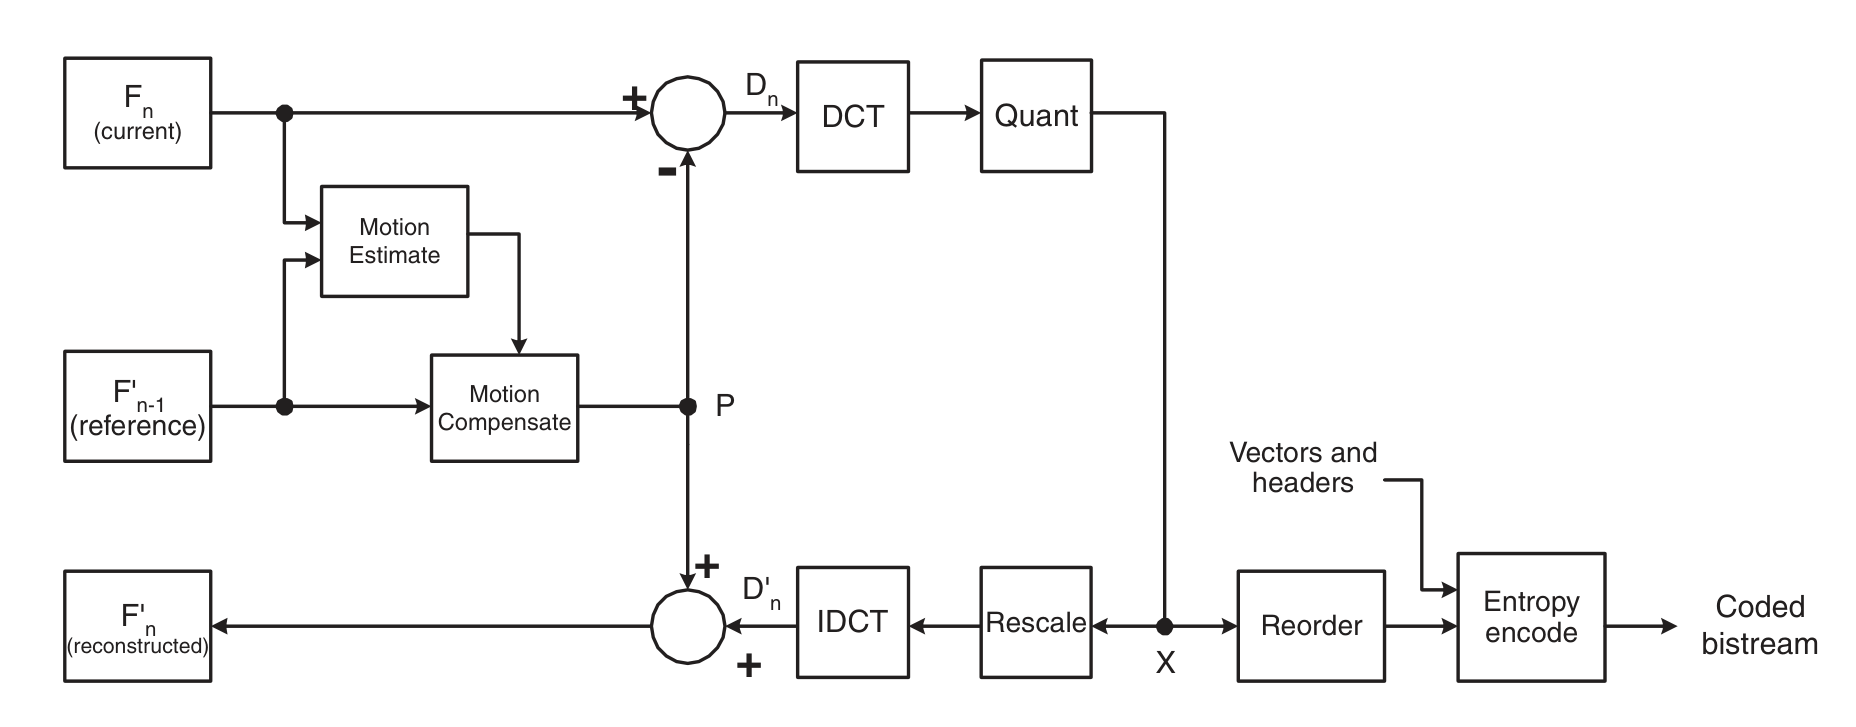
\includegraphics[width=\textwidth]{res/hybrid_codec_detailed.png}
	
	\caption{Detailed hybrid codec architecture.\cite{h264}}
	\label{fig:codec_highlevel}
\end{figure}

%The transform converts the samples into another domain in which they are represented by transform coefficients. The coefficients are quantized to remove insignificant values, leaving a small number of significant coefficients that provide a more compact representation of the residual frame. The output of the spatial model is a set of quantized transform coefficients.

%The parameters of the prediction model, i.e. intra prediction mode(s) or inter prediction mode(s) and motion vectors, and the spatial model, i.e. coefficients, are compressed by the entropy encoder. This removes statistical redundancy in the data, for example representing commonly occurring vectors and coefficients by short binary codes. The entropy encoder produces a compressed bit stream or file that may be transmitted and/or stored. A compressed sequence consists of coded prediction parameters, coded residual coefficients and header information. The video decoder reconstructs a video frame from the compressed bit stream. The coefficients and prediction parameters are decoded by an entropy decoder after which the spatial model is decoded to reconstruct a version of the residual frame. The decoder uses the prediction parameters, together with previously decoded image pixels, to create a prediction of the current frame and the frame itself is reconstructed by adding the residual frame to this prediction.

The output of a hybrid video encoder is a \textit{bit stream} (or \textit{bitstream}), i.e. a compressed sequence of coded residual coefficients and other parameters. The decoder applies the same process inversely in order to reconstruct the original video frames, with some approximation.

\subsection{Frame types and GOP}
\label{sec:bg/compression/gop}

As we have seen, the prediction model can be based on temporal (inter-frame) prediction or spatial (intra-frame) prediction. The type of prediction that is used and which reference frames are used for the prediction determine the type of frame. In particular:

\begin{itemize}
    \item \textbf{I-frames} (\textit{Intra-frames}) are frames that do not require any other frames to be decoded and are thus compressed only through intra-frame prediction.
    \item \textbf{P-frames} (\textit{Predicted frames}) are frames that can reference other previous frames when performing temporal prediction. Depending on the codec, a frame can reference one or more previous frames.
    \item \textbf{B-frames} (\textit{Bi-directional predicted frames}) are frames that can reference both previous and future frames as reference frames in temporal prediction. They are more computationally expensive to encode, but are usually the most compressible ones.
\end{itemize}

Because of inter-frame dependencies, the display order of frames is very often different from the decoding order.

Depending on the type of frames that are used to encode a video sequence, different \textbf{prediction structures} can be obtained. For example, low delay applications could use a structure like the one in figure \ref{fig:codec_gop1}, where only I-frames and P-frames are used and P-frames always reference the previous frame. I-frames need to be inserted in the stream every now and then to allow more efficient random access (\textit{seeking}). Another reason is that in some cases scene cuts might justify the use of an I-frame instead of a P-frame, depending on how drastic the scene change is.

\begin{figure}
	\centering
	
	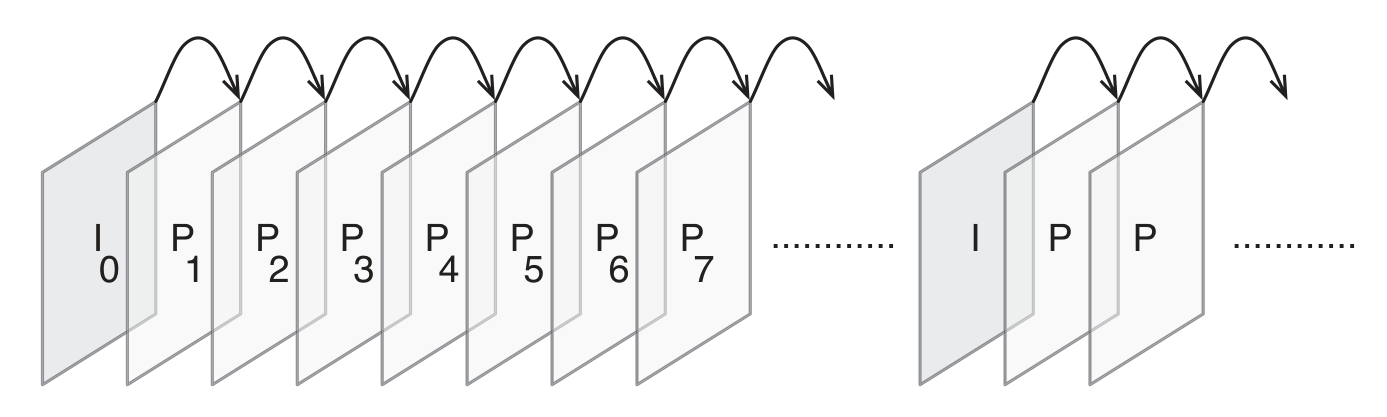
\includegraphics[width=0.9\textwidth]{res/gop1.png}
	
	\caption{Simple GOP structure with no B-frames.}
	\label{fig:codec_gop1}
\end{figure}

Most of the time, the arrangement of the frames is much more complex and is usually defined by a \textbf{Group of Pictures (GOP)} structure, as seen in Figure \ref{fig:codec_gop2}. A GOP always starts with an I-frame and is most of the time \textit{closed}, which means that it is independent from previous and future GOPs. As a consequence, in a closed-GOP scenario the decoder does not need access to previous of future GOPs to be able to decode frames in the current GOP.

The structure of a GOP can be summarized as a string sequence, like \texttt{IBBPBBPBBPBBI}, or through two numbers, \texttt{M} and \texttt{N}, that respectively determine the distance between P-frames, and the GOP size. For example, the structure in Figure \ref{fig:codec_gop2} can be expressed as \texttt{M=3, N=12}.

\begin{figure}
	\centering
	
	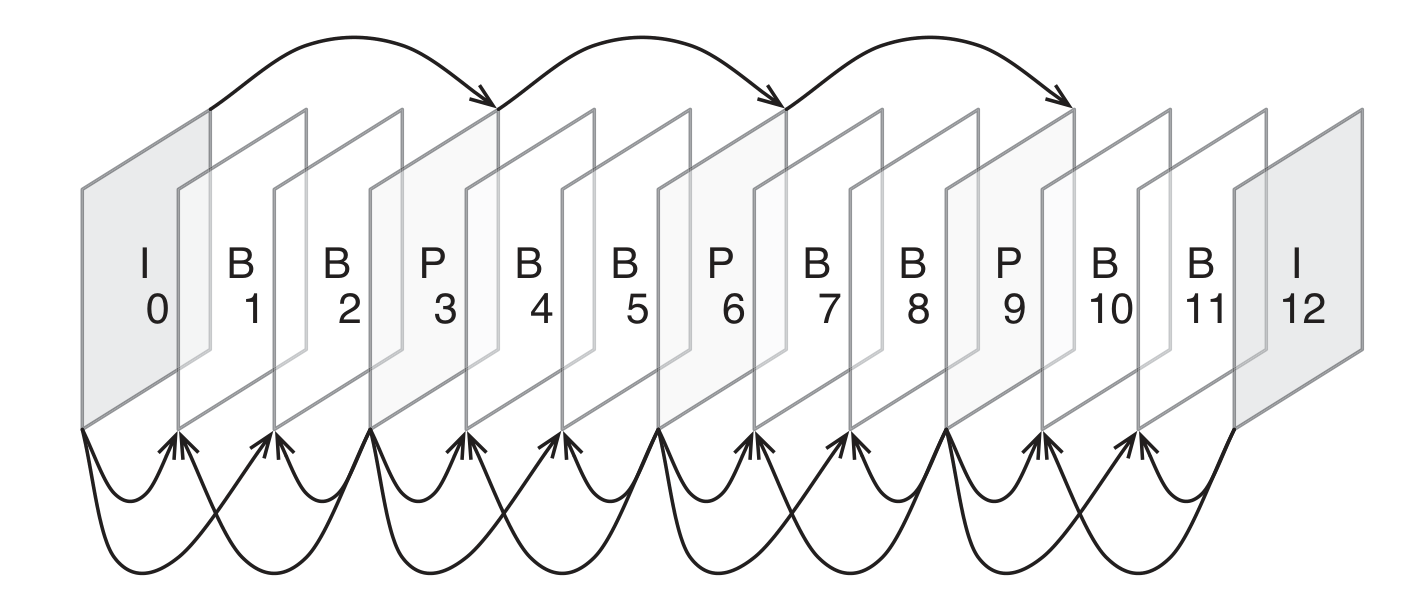
\includegraphics[width=0.8\textwidth]{res/gop2.png}
	
	\caption{Typical GOP structure, \texttt{M=3, N=12}.}
	\label{fig:codec_gop2}
\end{figure}

\subsection{Popular video codecs}
\label{sec:bg/compression/codecs}


% H.264
% only the decoding formats
% annex B
% profiles/levels

\subsection{Container formats}

\section{Audio compression}
\label{sec:bg/audio}



\section{A typical live streaming architecture}
\label{sec:bg/compression}

\section{Adaptive bitrate technologies}
\label{sec:bg/technologies}


